\documentclass[UTF8,a4paper,11pt,fontset=fandol]{ctexart}
\usepackage{geometry}
\geometry{margin=2.2cm}
\usepackage{amsmath,amssymb,longtable,booktabs,array,hyperref,xcolor,enumitem,graphicx,float}
\hypersetup{colorlinks=true,linkcolor=blue,urlcolor=blue}
\setlist[itemize]{leftmargin=1.3em,itemsep=0.2em}
\definecolor{notegray}{RGB}{246,248,251}
\title{P06. Eco-driving for Electric Connected Vehicles at Signalized Intersections: A Parameterized Reinforcement Learning Approach\\中英双语博士精读笔记}
\author{Xia Jiang; Jian Zhang; Dan Li}
\date{2023 · Journal article related DOI / arXiv version}
\begin{document}
\maketitle

\noindent\textbf{Theme / 主题：} Electric CV eco-driving + parameterized RL\\
\textbf{Method family / 方法族：} Parameterized reinforcement learning / 参数化强化学习\\
\textbf{PDF pages / 页数：} 27 \quad
\textbf{Relevance / 相关度：} 83/100\\
\textbf{Source / 来源：} \url{https://arxiv.org/abs/2206.12065}

\section{论文全景速览与核心贡献 / High-Level Overview \& Core Contributions}
\subsection{研究背景与痛点 / Background \& Pain Points}
这篇论文位于“Electric CV eco-driving + parameterized RL”方向。对你的 JSSP-based Intersection Management 课题，它回答的是高层调度、低层轨迹平滑、安全过滤或真实验证中的一个关键子问题：如何让车辆在路口少停、少冲突、少能耗，同时保持在线可执行。

The paper belongs to the theme of Electric CV eco-driving + parameterized RL. For a JSSP-based intersection-management thesis, it illuminates one of the key layers: scheduling, smoothing, safety filtering, or real-world validation.

\textbf{Pain point / 痛点：} Signalized intersections and electric connected vehicles rather than fully signal-free autonomous scheduling.

\subsection{核心科学问题 / Core Scientific Question}
如何同时处理离散驾驶决策和连续控制参数，使电动网联车在信号交叉口实现节能通行？

How can discrete maneuver choices and continuous control parameters be learned jointly for EV eco-driving at signalized intersections?

\subsection{科学贡献 / Scientific Contributions}
\begin{itemize}
\item 方法贡献 (method contribution)：Parameterized RL combines model-based car-following, lane-changing policy, and learned longitudinal/lateral decisions.
\item 安全/避碰贡献 (safety contribution)：Safety is handled through model-based car-following and lane-changing constraints around human-driven vehicles.
\item 平滑/停止避免贡献 (smoothing contribution)：Learns energy-saving actions around signalized intersections without interrupting surrounding HDVs.
\item 创新力度评判 (reviewer judgement)：中等偏强：参数化动作空间贴合驾驶决策结构，对混合离散-连续调度有启发。
\end{itemize}


\subsection{核心概念对照 / Core Concepts}
\begin{longtable}{p{0.24\linewidth}p{0.28\linewidth}p{0.40\linewidth}}
\toprule
中文概念 & English Concept & Role / 学术作用\\
\midrule
自动交叉口管理 & Autonomous Intersection Management & 把信号控制替换为车辆级调度与控制。 \\
轨迹平滑 & Trajectory Smoothing & 减少急加减速、停车和能耗峰值。 \\
安全约束 & Safety Constraints & 把碰撞风险写成距离、时间间隔或屏障函数。 \\
Parameterized reinforcement learning & 参数化强化学习 & 该论文的核心方法族。 \\
\bottomrule
\end{longtable}

\section{教材式学习路径与关键截图 / Textbook-Style Study Path \& PDF Snapshots}
\subsection{学习路径 / Study Path}
\begin{itemize}
\item 第一遍先读首页截图、摘要与引言，确认研究问题和场景假设。
\item 第二遍沿着技术路线图复现模型变量、约束和求解器输入输出。
\item 第三遍逐节阅读 section deep reading，对照 PDF 截图检查公式、图表和实验。
\item 第四遍只站在审稿人视角重读实验，判断 baseline、公平性、消融和鲁棒性。
\item 最后把博士 checklist 写成自己的复现实验或论文拓展计划。
\end{itemize}


\subsection{博士阅读 Checklist / Doctoral Reading Checklist}
\begin{itemize}
\item 能否独立重写核心公式：参数化动作 MDP / Parameterized-action MDP，并解释每个符号的物理意义？
\item 能否画出输入-模型-算法-控制-验证的数据流图？
\item 能否指出至少两个强假设，并说明它们在真实交通中何时失效？
\item 能否复述实验基准是否公平，指标是否覆盖效率、安全、能耗和计算时间？
\item 能否提出一个与自己 JSSP/RL/smoother 课题直接相连的拓展实验？
\end{itemize}


\subsection{关键截图讲解 / PDF Snapshot Explanation}
Screenshots are selected anchors from the local PDFs for study and parallel reading. They do not replace the original paper.

\begin{figure}[H]
\centering

\includegraphics[width=0.92\linewidth]{../../assets/P06_jiang2023ecodriving/01_title_and_abstract_p1.jpg}
\caption{首页与摘要 / Title and abstract page (p.1, full\_page). 这张截图用于把笔记中的抽象概念拉回原论文页面，便于你平行阅读原文、公式、图表和实验设置。 与当前课题的连接：Provides a SUMO-compatible example of energy and stop reduction metrics for the experimental section.}
\end{figure}

\begin{figure}[H]
\centering
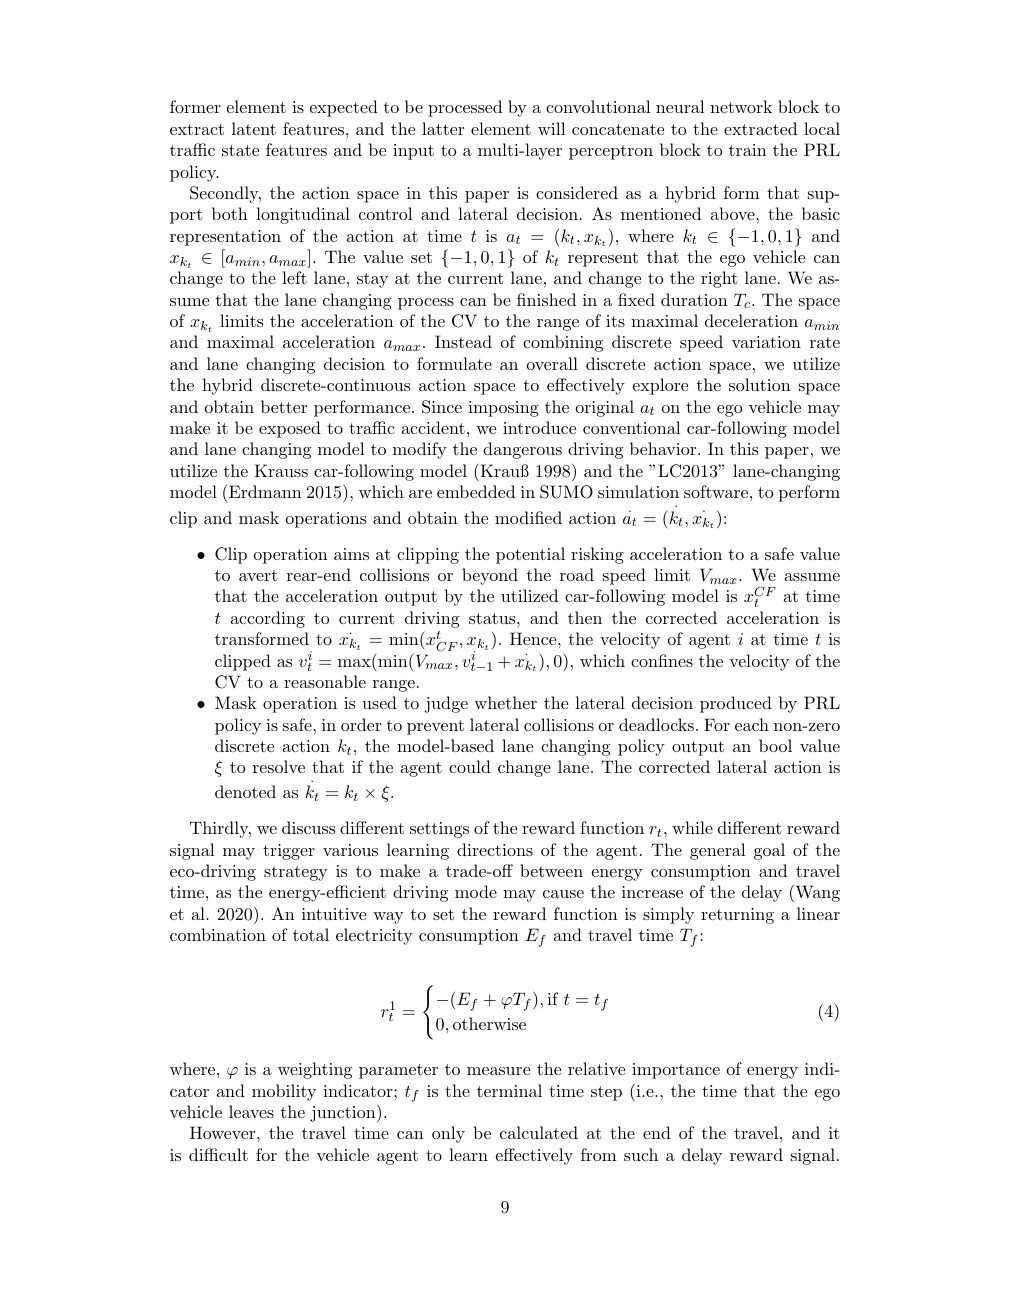
\includegraphics[width=0.92\linewidth]{../../assets/P06_jiang2023ecodriving/02_modeling_or_problem_setup_p9.jpg}
\caption{建模或问题设定页 / Modeling or problem-setup page (p.9, full\_page). 这张截图用于把笔记中的抽象概念拉回原论文页面，便于你平行阅读原文、公式、图表和实验设置。 与当前课题的连接：Provides a SUMO-compatible example of energy and stop reduction metrics for the experimental section.}
\end{figure}

\begin{figure}[H]
\centering
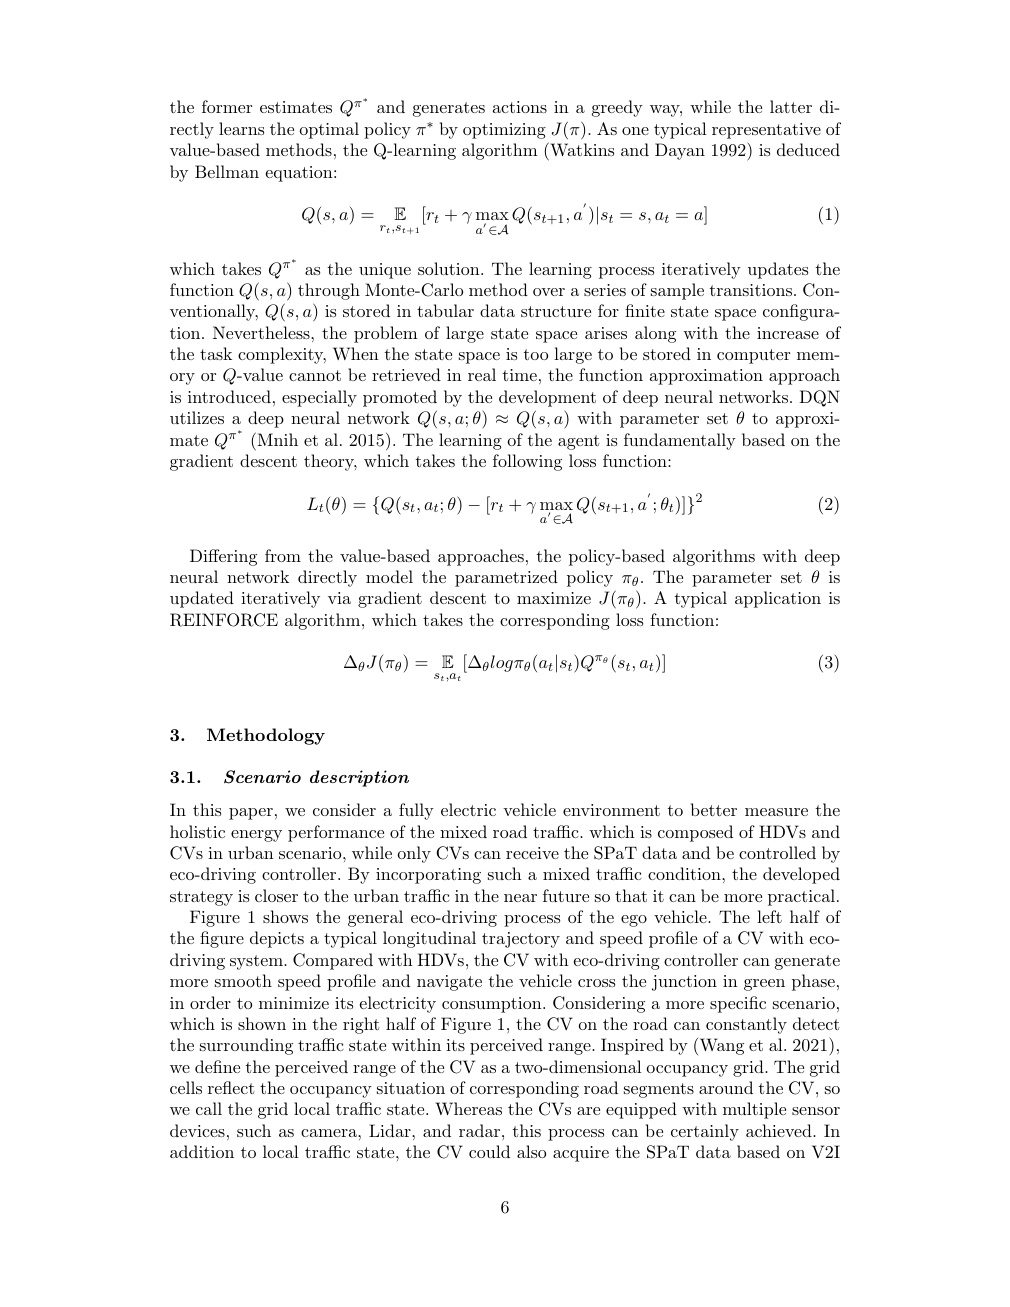
\includegraphics[width=0.92\linewidth]{../../assets/P06_jiang2023ecodriving/03_core_method_or_algorithm_p6.jpg}
\caption{核心方法或算法页 / Core method or algorithm page (p.6, full\_page). 这张截图用于把笔记中的抽象概念拉回原论文页面，便于你平行阅读原文、公式、图表和实验设置。 与当前课题的连接：Provides a SUMO-compatible example of energy and stop reduction metrics for the experimental section.}
\end{figure}

\begin{figure}[H]
\centering
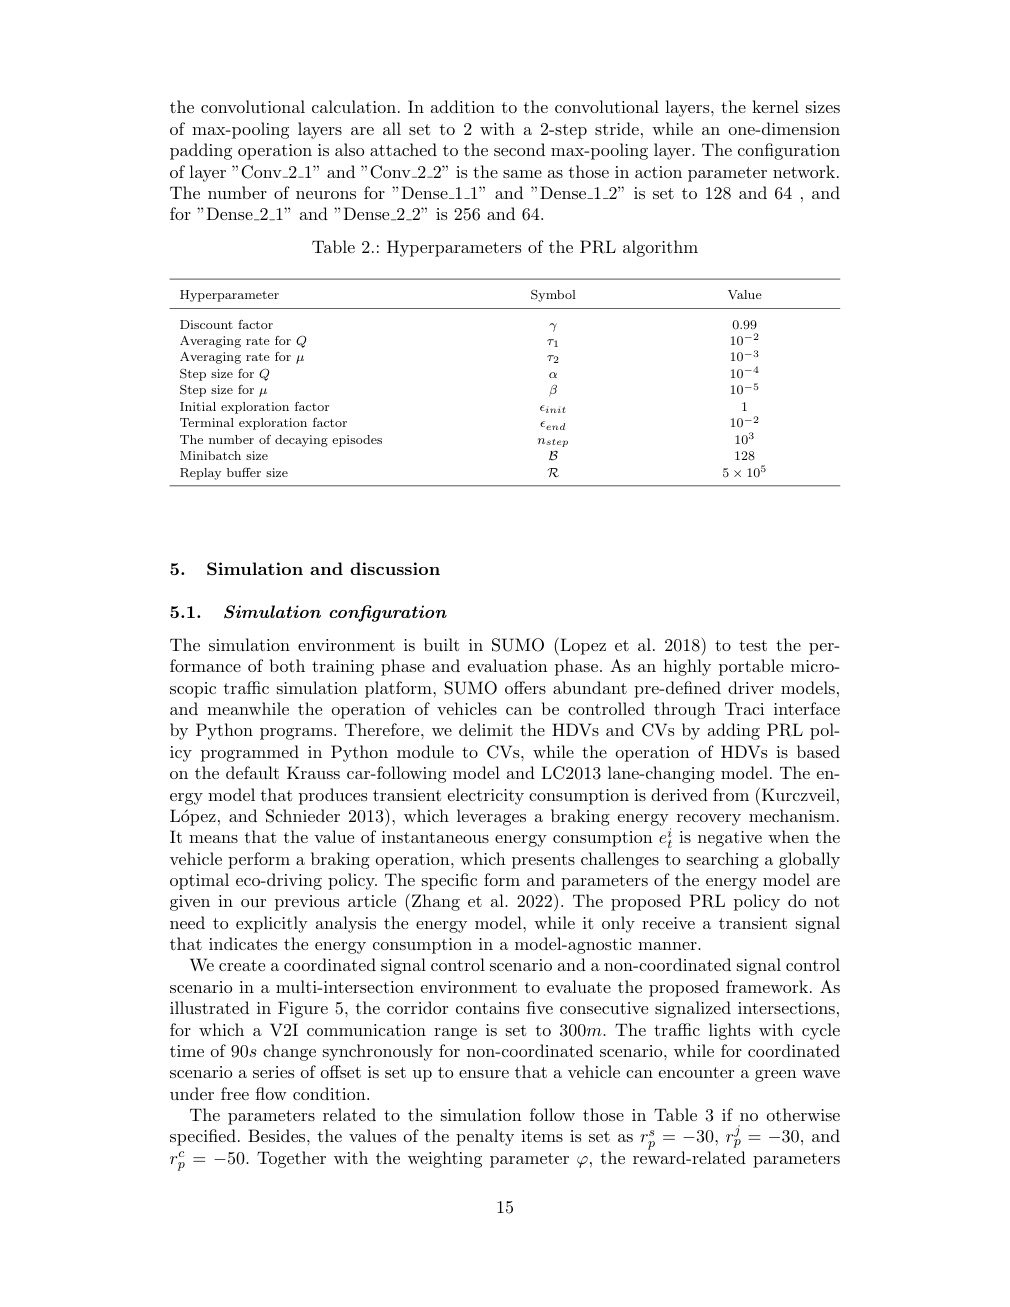
\includegraphics[width=0.92\linewidth]{../../assets/P06_jiang2023ecodriving/04_experiments_or_results_p15.jpg}
\caption{实验或结果页 / Experiments or results page (p.15, full\_page). 这张截图用于把笔记中的抽象概念拉回原论文页面，便于你平行阅读原文、公式、图表和实验设置。 与当前课题的连接：Provides a SUMO-compatible example of energy and stop reduction metrics for the experimental section.}
\end{figure}

\begin{figure}[H]
\centering
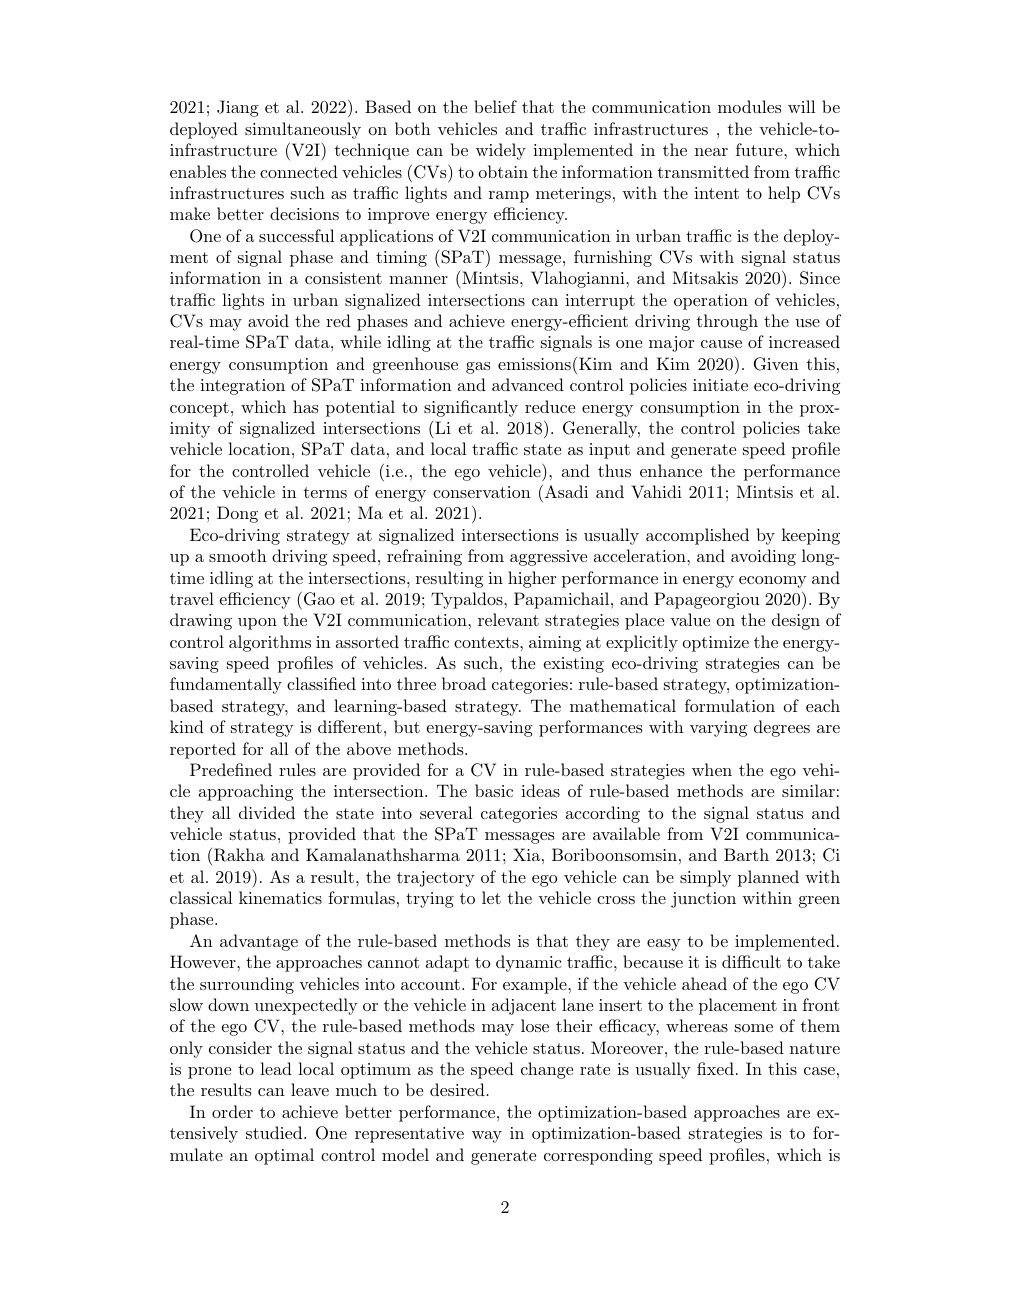
\includegraphics[width=0.92\linewidth]{../../assets/P06_jiang2023ecodriving/05_supplemental_reading_page_p2.jpg}
\caption{补充精读页 / Supplemental close-reading page (p.2, full\_page). 这张截图用于把笔记中的抽象概念拉回原论文页面，便于你平行阅读原文、公式、图表和实验设置。 与当前课题的连接：Provides a SUMO-compatible example of energy and stop reduction metrics for the experimental section.}
\end{figure}


\section{章节精读与逐段导读 / Section-by-Section Deep Reading \& Walkthrough}
\subsection*{p.1 1. Introduction}
\textbf{章节目标 / Learning goal：} 建立研究动机：为什么传统信号控制、FCFS 或单车控制不足以处理该论文关注的交叉口协同问题。

Understand why the paper needs a new coordination method rather than a standard signal, FCFS, or single-vehicle controller.

\textbf{关键论点 / Key argument：} 这一部分通常把痛点落到 Electric CV eco-driving + parameterized RL：既要提高效率，又要保持安全与在线可执行。

\textbf{技术焦点 / Technical focus：} 精读时标出作者批判的 baseline、场景假设、交通参与者类型和隐含优化目标。

\textbf{审稿追问 / Reviewer question：} 作者指出的痛点是否真的需要新方法，还是可以由更强的优化器/更保守规则解决？

\subsection*{p.5 2. Background of Reinforcement Learning}
\textbf{章节目标 / Learning goal：} 建立方法谱系和相关工作边界，避免把本文贡献误读为完全从零开始。

Place the paper inside the broader method taxonomy.

\textbf{关键论点 / Key argument：} 该部分说明作者站在哪些已有工作之上，以及本文选择绕开或继承了哪些限制。

\textbf{技术焦点 / Technical focus：} 把相关工作按 scheduler、smoother、safety filter、evaluation 四类重排。

\textbf{审稿追问 / Reviewer question：} 作者是否公平比较了最接近的强 baseline？

\subsection*{p.6 3. Methodology}
\textbf{章节目标 / Learning goal：} 解释算法如何把模型转化为可执行决策，并说明在线运行机制。

Trace how the paper turns the model into executable online decisions.

\textbf{关键论点 / Key argument：} 参数化 RL 把驾驶行为拆成离散模式和对应连续参数，结合模型式跟驰/变道规则处理周围 HDV，再用学习策略选择节能动作。该结构很适合未来把高层调度选择和低层连续轨迹合并。

\textbf{技术焦点 / Technical focus：} 画出输入、核心求解器、输出和安全检查接口，明确哪些步骤是优化、哪些是规则、哪些是学习。

\textbf{审稿追问 / Reviewer question：} 若算法某一步失败，论文有没有 fallback、重规划或安全过滤机制？

\subsection*{p.6 3.1. Scenario description}
\textbf{章节目标 / Learning goal：} 承接前后章节，补充局部定义、案例或实现细节。

Recover implementation details needed for reproduction.

\textbf{关键论点 / Key argument：} 这类章节常常不是主贡献，但决定你能否真正复现方法。

\textbf{技术焦点 / Technical focus：} 检查它是否给出了参数、伪代码、场景划分或实现细节。

\textbf{审稿追问 / Reviewer question：} 跳过该节会不会导致公式或实验无法复现？

\subsection*{p.7 3.2. Agent framework}
\textbf{章节目标 / Learning goal：} 解释算法如何把模型转化为可执行决策，并说明在线运行机制。

Trace how the paper turns the model into executable online decisions.

\textbf{关键论点 / Key argument：} 参数化 RL 把驾驶行为拆成离散模式和对应连续参数，结合模型式跟驰/变道规则处理周围 HDV，再用学习策略选择节能动作。该结构很适合未来把高层调度选择和低层连续轨迹合并。

\textbf{技术焦点 / Technical focus：} 画出输入、核心求解器、输出和安全检查接口，明确哪些步骤是优化、哪些是规则、哪些是学习。

\textbf{审稿追问 / Reviewer question：} 若算法某一步失败，论文有没有 fallback、重规划或安全过滤机制？

\subsection*{p.10 4. PRL for eco-driving}
\textbf{章节目标 / Learning goal：} 承接前后章节，补充局部定义、案例或实现细节。

Recover implementation details needed for reproduction.

\textbf{关键论点 / Key argument：} 这类章节常常不是主贡献，但决定你能否真正复现方法。

\textbf{技术焦点 / Technical focus：} 检查它是否给出了参数、伪代码、场景划分或实现细节。

\textbf{审稿追问 / Reviewer question：} 跳过该节会不会导致公式或实验无法复现？

\subsection*{p.10 4.1. Reinforcement Learning in Hybrid Action Space}
\textbf{章节目标 / Learning goal：} 承接前后章节，补充局部定义、案例或实现细节。

Recover implementation details needed for reproduction.

\textbf{关键论点 / Key argument：} 这类章节常常不是主贡献，但决定你能否真正复现方法。

\textbf{技术焦点 / Technical focus：} 检查它是否给出了参数、伪代码、场景划分或实现细节。

\textbf{审稿追问 / Reviewer question：} 跳过该节会不会导致公式或实验无法复现？

\subsection*{p.12 4.2. PRL algorithm}
\textbf{章节目标 / Learning goal：} 解释算法如何把模型转化为可执行决策，并说明在线运行机制。

Trace how the paper turns the model into executable online decisions.

\textbf{关键论点 / Key argument：} 参数化 RL 把驾驶行为拆成离散模式和对应连续参数，结合模型式跟驰/变道规则处理周围 HDV，再用学习策略选择节能动作。该结构很适合未来把高层调度选择和低层连续轨迹合并。

\textbf{技术焦点 / Technical focus：} 画出输入、核心求解器、输出和安全检查接口，明确哪些步骤是优化、哪些是规则、哪些是学习。

\textbf{审稿追问 / Reviewer question：} 若算法某一步失败，论文有没有 fallback、重规划或安全过滤机制？


\subsection{逐段式导读 / Paragraph-Level Walkthrough}
\paragraph{Opening motivation / 开篇动机段}先把作者的痛点翻译成一句博士问题：如何同时处理离散驾驶决策和连续控制参数，使电动网联车在信号交叉口实现节能通行？ 读这一段时不要急着接受动机，要追问传统 FCFS、信号灯或保守 MPC 为什么不足。

Turn the opening motivation into one doctoral-level question and test whether the paper truly needs a new method.

\paragraph{Assumption and setting / 假设与场景段}把车辆类型、通信条件、路口类型和动力学假设列成表。该文的关键边界包括：周围车辆行为可由跟驰/变道模型近似。；电动车能耗模型可靠，且可用于仿真奖励。；信号灯信息和车辆状态可观测。

List vehicle type, communication, intersection setting, and dynamics assumptions before reading the equations.

\paragraph{Model and notation / 模型与符号段}围绕核心公式“参数化动作 MDP / Parameterized-action MDP”复写符号表，确认每个变量是决策变量、状态变量、参数还是约束阈值。

Rewrite the symbol table around the core formulation and classify variables as states, decisions, parameters, or constraints.

\paragraph{Algorithm mechanism / 算法机制段}把算法读成一条数据流：输入交通状态，执行 Parameterized RL combines model-based car-following, lane-changing policy, and learned longitudinal/lateral decisions.，输出可执行通行/控制决策，并检查安全接口。

Read the algorithm as a dataflow from traffic state to executable sequence/control decision, with explicit safety interfaces.

\paragraph{Experiment and evidence / 实验证据段}不要只看作者报告的提升，要检查基准、公平性和指标。本文验证描述为：SUMO evaluation from single-vehicle and flow perspectives.

Go beyond reported gains and inspect baselines, fairness, metrics, and computation time.

\paragraph{Reviewer synthesis / 审稿式总结段}最后把贡献拆成可发表与需补强两部分。对你课题最直接的用途是：Provides a SUMO-compatible example of energy and stop reduction metrics for the experimental section.

Separate publishable contribution from missing evidence, then connect the result to your own thesis architecture.


\section{技术路线图与贡献量评估 / Technical Route \& Contribution Matrix}
\begin{longtable}{p{0.08\linewidth}p{0.24\linewidth}p{0.58\linewidth}}
\toprule
Step & Stage / 阶段 & Content / 内容\\
\midrule
1 & 输入 / Input & 车辆状态、路径/车道、交通需求、信号或协同信息。 \\
2 & 建模 / Modeling & 参数化动作 MDP / Parameterized-action MDP \\
3 & 核心求解 / Core solver & Parameterized RL combines model-based car-following, lane-changing policy, and learned longitudinal/lateral decisions. \\
4 & 安全接口 / Safety interface & Safety is handled through model-based car-following and lane-changing constraints around human-driven vehicles. \\
5 & 平滑与效率 / Smoothing and efficiency & Learns energy-saving actions around signalized intersections without interrupting surrounding HDVs. \\
6 & 验证 / Validation & SUMO evaluation from single-vehicle and flow perspectives. \\
\bottomrule
\end{longtable}

\begin{longtable}{p{0.34\linewidth}p{0.14\linewidth}p{0.42\linewidth}}
\toprule
Dimension / 维度 & Score & Comment / 评语\\
\midrule
理论贡献 / Theoretical contribution & 3/5 & 参数化动作 MDP / Parameterized-action MDP \\
算法贡献 / Algorithmic contribution & 4/5 & Parameterized RL combines model-based car-following, lane-changing policy, and learned longitudinal/lateral decisions. \\
实验贡献 / Experimental contribution & 3/5 & SUMO evaluation from single-vehicle and flow perspectives. \\
工程贡献 / Engineering contribution & 3/5 & Safety is handled through model-based car-following and lane-changing constraints around human-driven vehicles. \\
博士课题价值 / PhD relevance & 4/5 & Provides a SUMO-compatible example of energy and stop reduction metrics for the experimental section. \\
\bottomrule
\end{longtable}

\section{理论方法论深度解构 / Methodology \& Theoretical Framework}
\subsection{问题数学建模 / Mathematical Formulation}
\textbf{参数化动作 MDP / Parameterized-action MDP}
\[
a_t=(d_t,\xi_t),\quad d_t\in\mathcal{D},\;\xi_t\in\mathbb{R}^{m(d_t)},\quad Q(s_t,d_t,\xi_t)\approx \mathbb{E}[R_t]
\]
\begin{longtable}{p{0.16\linewidth}p{0.25\linewidth}p{0.25\linewidth}p{0.25\linewidth}}
\toprule
Symbol / 符号 & 含义 & Meaning & Role / 建模作用\\
\midrule
d\_t & 离散驾驶决策 & discrete driving decision & 如保持、变道、跟驰模式 \\
xi\_t & 连续动作参数 & continuous action parameter & 如目标速度或加速度幅值 \\
D & 离散动作集合 & discrete action set & 描述可选机动 \\
Q & 动作价值函数 & action-value function & 评价离散-连续组合收益 \\
R\_t & 回报 & return & 累积能耗、效率和安全目标 \\
\bottomrule
\end{longtable}

\subsection{核心算法架构 / Core Algorithm Layout}
参数化 RL 把驾驶行为拆成离散模式和对应连续参数，结合模型式跟驰/变道规则处理周围 HDV，再用学习策略选择节能动作。该结构很适合未来把高层调度选择和低层连续轨迹合并。

Parameterized RL separates maneuver selection from continuous parameter control, combining learned decisions with model-based car-following and lane-changing constraints.

\subsection{收敛性、稳定性或实时性 / Convergence, Stability, Real-Time Feasibility}
模型式规则给安全留出底线，学习器主要优化效率和能耗；但混合动作空间训练难度较高，参数边界设计会影响收敛。

Model-based constraints provide a safety floor, while the learner optimizes energy and efficiency; convergence depends strongly on action parameterization.

\subsection{潜在假设与边界条件 / Assumptions \& Boundary Conditions}
\begin{itemize}
\item 周围车辆行为可由跟驰/变道模型近似。
\item 电动车能耗模型可靠，且可用于仿真奖励。
\item 信号灯信息和车辆状态可观测。
\end{itemize}


\section{实验验证与结果评判 / Experimental Validation \& Result Evaluation}
\textbf{Baselines \& Environment / 基准与环境：} 传统生态驾驶、普通 DQN/DDPG、规则驾驶、无参数化 RL 和 IDM。

\textbf{Validation / 验证：} SUMO evaluation from single-vehicle and flow perspectives.

\textbf{Metrics / 指标：} 电耗、平均速度、延误、停车次数、舒适性和混合交通影响。

\textbf{Ablation / 消融：} 应比较参数化 RL 与纯离散、纯连续动作策略；还应测试参数边界和模型式安全规则的贡献。

\textbf{Reviewer reading / 审稿式阅读提醒：} 阅读实验时不要只看平均值；应检查交通密度、车流方向、随机种子、失败案例和计算耗时。For doctoral reading, inspect density regimes, demand patterns, random seeds, failure cases, and computation time rather than only mean improvements.

\subsection{图表阅读线索 / Figure and Table Reading Cues}
PDF extraction detected approximately 33 figure references and 8 table references. Exact captions remain in the original PDF; the bilingual cues below tell you what to inspect first.

\begin{longtable}{p{0.24\linewidth}p{0.30\linewidth}p{0.36\linewidth}}
\toprule
图表名称 & Figure/Table Name & Reading focus / 阅读重点\\
\midrule
系统框架图 & system framework diagram & 先确认输入、决策层、控制层和安全约束之间的数据流。 \\
策略网络/训练流程图 & policy-network or training-pipeline diagram & 检查状态、动作、奖励、经验回放和安全惩罚是否闭环一致。 \\
实验指标对比图表 & experimental metric comparison plots/tables & 重点看平均值之外的密度变化、失败场景、计算时间和方差。 \\
\bottomrule
\end{longtable}

\section{审稿人视角：批判性思考与未来方向 / Critical Thinking \& Future Directions}
\subsection{论文局限性 / Limitations \& Weaknesses}
\begin{itemize}
\item 信号交叉口和电动车设定使结论不完全适用于无信号 CAV 调度。
\item 参数化动作设计依赖专家经验。
\item 混合交通中 HDV 模型错误可能传播到策略学习。
\end{itemize}


\subsection{博士课题拓展点 / Research Extensions for PhD}
\begin{itemize}
\item 把 JSSP 的车辆排序作为离散动作，把目标时间/速度作为连续参数。
\item 加入不确定 HDV 模型集合，做鲁棒参数化 RL。
\item 用分层策略把 lane choice、arrival time 和 speed profile 分别建模。
\end{itemize}


\subsection{如何服务当前课题 / Use in This Project}
Provides a SUMO-compatible example of energy and stop reduction metrics for the experimental section.

\section{交互式可视化与 PDF 排版蓝图 / Interactive Visualization \& PDF Layout Blueprint}
\textbf{动态参数 / Parameter：} CAV渗透率 / CAV penetration rate, range [0.05, 1.0] .

渗透率提高通常增强节能协同，但低渗透率下收益受 HDV 约束明显。

Higher penetration improves eco-coordination, while low penetration is constrained by HDVs.

\subsection{HTML 结构化布局建议 / HTML Structuring}
\begin{itemize}
\item 顶部固定 metadata bar：题名、作者、年份、主题、PDF 页数。
\item 左侧目录/section navigator，右侧为五大精读模块。
\item 公式卡片使用 <pre> 或 LaTeX block，紧跟符号表。
\item 审稿人批注用 reviewer-note block，博士拓展用 research-idea list。
\item 交互参数用 input[type=range] + canvas 曲线，打印 PDF 时隐藏交互控件但保留解释。
\end{itemize}


\section{来源锚点与逐节阅读路径 / Source Anchors \& Section-by-Section Reading Map}
\begin{longtable}{p{0.14\linewidth}p{0.76\linewidth}}
\toprule
Page & Extracted heading\\
\midrule
p.1 & 1. Introduction \\
p.6 & 3. Methodology \\
p.15 & 5. Simulation and discussion \\
\bottomrule
\end{longtable}

\paragraph{p.1 1. Introduction}定位问题背景、研究缺口和为什么现有保守/非协同方法不足。 / Frames the motivation, research gap, and limits of conservative or non-cooperative methods.

\paragraph{p.5 2. Background of Reinforcement Learning}作为局部论证段落阅读，关注它如何服务主问题。 / Read as a local argument and ask how it supports the main question.

\paragraph{p.6 3. Methodology}给出算法流程和求解机制，应重点追踪输入、输出和安全接口。 / Gives the algorithmic mechanism; track inputs, outputs, and safety interfaces.

\paragraph{p.6 3.1. Scenario description}作为局部论证段落阅读，关注它如何服务主问题。 / Read as a local argument and ask how it supports the main question.

\paragraph{p.7 3.2. Agent framework}给出算法流程和求解机制，应重点追踪输入、输出和安全接口。 / Gives the algorithmic mechanism; track inputs, outputs, and safety interfaces.

\paragraph{p.10 4. PRL for eco-driving}作为局部论证段落阅读，关注它如何服务主问题。 / Read as a local argument and ask how it supports the main question.

\paragraph{p.10 4.1. Reinforcement Learning in Hybrid Action Space}作为局部论证段落阅读，关注它如何服务主问题。 / Read as a local argument and ask how it supports the main question.

\paragraph{p.12 4.2. PRL algorithm}给出算法流程和求解机制，应重点追踪输入、输出和安全接口。 / Gives the algorithmic mechanism; track inputs, outputs, and safety interfaces.


\end{document}
